\chapter{Método Empírico}

Esquematicamente, o método empírico pode ser descrito por cinco fases:
\begin{enumerate}
\item {\em Observação:} medições sobre algum aspecto do mundo
\item {\em Hipótese:} concepção de um modelo consistente com as observações
\item {\em Predição:} eventos são previstos de acordo com o modelo
\item {\em Verificação:} as predições são testadas fazendo-se novas observações
\item {\em Validação:} o processo se repete ajustando o modelo até que ele concorde com as observações
\end{enumerate}

Dois pontos centrais sobre o método empírico é que as verificações devem ser {\em reprodutíveis} e as hipóteses {\em falseáveis}.
Uma hipóstese que não pode ser falseada por observações (empíricamente) não é científica e a o processo de verificação deve poder ser feito por outros cientístas independentes.

O aspecto do mundo que pretendemos investigar nesta disciplina é o tmepo de processamento de um algoritmo.
Lembre-se, porém, que um algoritmo é uma ideia que precede o advento dos computadores.
O algoritmo de Euclídes, por exemplo, data de 300 a.C., ou seja, séculos antes dos primeiros computadores começarem a ser construídos nos anos 40.
Embora o algoritmo seja um conceito matemático, uma série de pesquisadores tiveram a ideia de investigá-los de maneira empírica no final dos anos 60.
A série de livros The Art of Programing, de Donald Knuth, é um marco dessa abordagem dos estudos de algoritmos \cite{knuth97}.

Em nosso recorte, observaremos o tempo de processamento da execução de um programa para diferentes entradas.
Considere, por exemplo, o algoritmo para o problema da Busca apresentado no capítulo anterior:

\begin{codebox}
\Procname{$\proc{BuscaSequencial}(A, b)$}
\li \For $i \gets 1$ até $n$
\li \Do \If $a_i = b$
\li     \Then \Return $i$
        \End
    \End
\li \Return $\bot$
\End
\end{codebox}

Vamos implementar esse algoritmo na linguagem C de maneira direita:

\begin{lstlisting}[language=C]
  // devolve a posicao de n no arranjo ou -1 se nao encontrar
  int buscasequencial(int* array, int n, int size){
    int i;
    for(i = 0; i < size; i++)
      if(array[i] == n)
        return i;
    return -1;
  }      
\end{lstlisting}

Realizamos observações usando uma máquina específica (um notebook Dell com processador intel core i7 de $8^a$ geração de 1,9GHz) em um sistema operacional específico (Linux 5.11).
Medimos o tempo total de 300 buscas mal sucedidas em arranjos de tamanhos diferentes com valores inteiros positivos calculados aleatoriamente\footnote{Mais precisamente os valores seguem uma sequência pseudo-aleatória partindo de uma semente incial.}.
Os programas que calcula o tempo da busca e que gera as entradas estão disponíveis em \url{https://github.com/marciomr/IAA}.
Variamos o tamanho do arranjo entre um milhão e dez milhões.
Obtivemos o seguinte resultado para dez observações:

\begin{table}
  \label{tab:observacao}
  \begin{tabular}{|c|c|}
    \hline
    tamanho do arranjo em milhões & tempo de 300 buscas em segundos \\
    \hline 
    1                             & 0,99                            \\
    2                             & 2,08                            \\
    3                             & 3,12                            \\
    4                             & 3,99                            \\
    5                             & 5,05                            \\
    6                             & 5,94                            \\
    7                             & 7,03                            \\
    8                             & 7,92                            \\
    9                             & 8,93                            \\
    10                            & 9,85                            \\
    \hline
  \end{tabular}
\end{table}

As observações sugerem que para cada um milhão de valores no arranjo, o tempo de processamento aumenta mais ou menos um segundo.
Essa poderia ser nossa hipótese, mas podemos fazer algo um pouco mais sofisticado.
Vamos plotar os valores da tabela em um gráfico (Figura \ref{fig:observacao}).

\begin{figure}[htp]
  \label{fig:observacao}
  \includegraphics[width=0.9\textwidth]{imagens/grafico1.png}
  \caption{Tempo de processamento da busca sequencial.}
\end{figure}

Como os pontos estão mais ou menos alinhados e como é razoável supor que um arranjo sem nenhum elemento retornaria instantaneamente o resultado, faremos a hipótese de que o tempo de processamento segue uma função linear partindo do zero.
Ou seja, a seguinte função descreve o tempo de processamento da nossa implementação em nosso ambiente:

\begin{displaymath}
t(x) = a.x
\end{displaymath}

Podemos então usar uma regressão linear para estimar o valor de $a$ que minimize a distância desse reta para cada um dos pontos.
Obtemos então o valor $a = 0,997$.
Na Figura \ref{fig:hipotese} plotamos a função $t(x) = 0,997x$ no gráfico anterior.

\begin{figure}[htp]
  \label{fig:hipotese}
  \includegraphics[width=0.9\textwidth]{imagens/grafico2.png}
  \caption{Gráfico ilustrando a hipótese de que o tempo de processamento da busca sequencial segue a função linear $t(x) = 0,997x$.}
\end{figure}

Podemos agora testar nossa hipótese de que o tempo de processamento da nossa implementação da busca sequencial para outros valores ainda não observados.
A segunda coluna da Tabela \ref{tab:verificacao} mostra os valores previstos pela hipótese para o tempo de processamento para entradas de tamanho 11 a 15 milhões.
Finalmente, podemos testar a hipótese.
Na última coluna da mesma tabela indicamos os valores observados para essas entradas:

\begin{table}
  \label{tab:verificacao}
  \begin{tabular}{|c|c|c|}
    \hline
    tamanho do arranjo em milhões & tempo previsto & tempo observado \\
    \hline 
    11                             & 10,97         & 10,87           \\
    12                             & 11,97         & 11,81           \\
    13                             & 12,97         & 12,78           \\
    14                             & 13,96         & 14,00           \\
    15                             & 14,96         & 14,74           \\
    \hline
  \end{tabular}
  \caption{Tempo de processamento previsto e observado para tamanhos maiores de arranjos.}
\end{table}

Os valores observados são notavelmente próximos aos previstos.
Ou seja, nossa hipótese foi verificada.
Poderíamos neste momento utilizar um teste estatístico para verificar nossa hipótese, mas isso foge do escopo desta disciplina.
Por hora diremos apenas que os dados parecem verificar a hipótese.

Consideremos agora a seguinte versão modificada do Problema da busca:

\vspace{0.5cm}

{\bf Problema da busca em uma sequência ordenada}\\

{\bf Entrada:} Uma sequência de $n$ valores $a_1, \dots, a_n$ em ordem crescente, isto é, $a_i \leq a_j$ para todo $i \leq j$ e $b \in \mathbb{Z}$.\\

{\bf Saída:} $i \in \mathbb{N}$ tal que $a_i = b$ se existir ou $\bot$ caso contrário.

\vspace{0.5cm}

Note que este problema é uma versão restrita do problema anterior.
Assim, toda solução do Problema da busca é também uma solução para o Problema da busca em uma sequência ordenada -- o inverso não é necessariamente verdadeiro.
Em particular, o algoritmo de Busca Sequêncial resolve ambos os problemas.
O seguinte algoritmo, por sua vez, resolve apenas o segundo:

\begin{codebox}
  \Procname{$\proc{BuscaBinaria}(A, b)$}
  \li \Comment Recebe uma sequência ordenada $a_1, \dots a_n$ e um valor $b$ todos inteiros
  \li \Comment Devolve $i$ tal que $a_i = b$ ou $\bot$ caso $b$ não ocorra na sequência
  \li $i \gets 1$
  \li $j \gets |A|$
  \li \While $i \leq j$
  \li \Do $m \gets \left \lfloor{\frac{j+i}{2}}\right\rfloor$
  \li \If $b < a_m$
  \li     \Then $j \gets m - 1$
  \li \Else
      \If $b > a_m$
  \li      \Then $i \gets m + 1$
  \li \Else \Return m 
      \End
  \End
  \End
  \li \Return $\bot$
\end{codebox}

Este algoritmo é um pouco mais sofisticado do que o anterior.
Começamos avaliando o elemento no centro da sequência ($a_m$).
Como a sequência está em ordem crescent, se o valor procurado ($b$) for maior do que $a_m$ então ele deve estar depois do valor central e podemos ignorar todos os valores anteriores a $m$.
Analogamente, se $b$ for menor que $a_m$ ele deve estar antes de $m$ e podemos ignorar todos os valores posteriores.

Como fizemos no exemplo anterior, vamos avaliar o tempo de processamento deste algoritmo utilizando o método empírico.
O primeiro passo é fazer algumas observações.
Vamos repetir as observações feitas no exemplo anterior.

\begin{table}
  \label{tab:observacao2}
  \begin{tabular}{|c|c|}
    \hline
    tamanho do arranjo em milhões & tempo de 300 buscas em segundos \\
    \hline 
    1                             & 0,00                            \\
    2                             & 0,00                            \\
    3                             & 0,00                            \\
    4                             & 0,00                            \\
    5                             & 0,00                            \\
    6                             & 0,00                            \\
    7                             & 0,00                            \\
    8                             & 0,00                            \\
    9                             & 0,00                            \\
    10                            & 0,00                            \\
    \hline
  \end{tabular}
\end{table}

As observações sugerem que o novo algoritmo é muito mais eficiente do que o primeiro.
Porém, elas não nos ajudam a conceber um modelo.

Façamos então observações com mais repetições.
Depois de alguns testes aprendemos que repetindo dez milhões de buscas o tempo de processamento passa a ser mensurável.

\begin{table}
  \label{tab:observacao3}
  \begin{tabular}{|c|c|}
    \hline
    tamanho do arranjo em milhões & tempo de 10M buscas em segundos \\
    \hline 
    1                             & 0,66                            \\
    2                             & 0,64                            \\
    3                             & 0,60                            \\
    4                             & 0,59                            \\
    5                             & 0,62                            \\
    6                             & 0,63                            \\
    7                             & 0,63                            \\
    8                             & 0,63                            \\
    9                             & 0,66                            \\
    10                            & 0,65                            \\
    \hline
  \end{tabular}
\end{table}

Desta vez conseguimos fazer as medições.
As observações sugerem que o tempo de processamento é independente do tamanho do arranjo.
Para arranjos de qualquer tamanho o tempo de procesamento parece ser maior ou menos o mesmo.
Podemos então levantar a hipótese de que o tempo de processamento é constante:

\begin{displaymath}
  t(x) = a
\end{displaymath}

Para calcular o valor de $a$ peguemos a média das observações $a = 0,63$.

\begin{figure}[htp]
  \label{fig:hipotese2}
  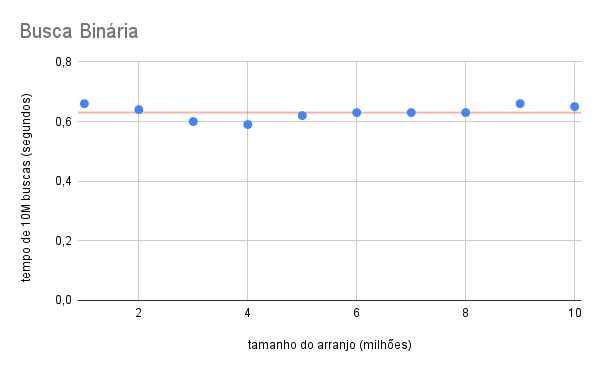
\includegraphics[width=0.9\textwidth]{imagens/grafico3.png}
  \caption{Gráfico ilustrando a hipótese de que o tempo de processamento da busca binária segue a função constante $t(x) = 0,63$.}
\end{figure}

Assim, nosso modelo preveria que para entradas de qualquer tamanho, o tempo de processamento seria próximo a $0,63$ segundos.
Vamos testar essa hipótese com entradas de tamanhos bem maior para ver se a hipótese se verifica.

\begin{table}
  \label{tab:verificacao}
  \begin{tabular}{|c|c|c|}
    \hline
    tamanho do arranjo em milhões & tempo previsto & tempo observado \\
    \hline 
    20                            & 0,63           & 0,68            \\
    100                           & 0,63           & 0,75            \\
    500                           & 0,63           & 0,81            \\
    1000                          & 0,63           & 0,89            \\
    \hline
  \end{tabular}
  \caption{Tempo de processamento previsto e observado para tamanhos maiores de arranjos.}
\end{table}

O processamento continua muito rápido mesmo para arranjos bem grandes, mas parece que a hipótese não foi verificada.
Seguindo o método empírico, devemos fazer novas observações para tentar formular uma nova hipótese.
Tentemos repetir nossas observações com uma maior amplitude de valores.
Ao invés de aumentar o tamanho de nossa sequência em um tamanho fixo a cada observação, vamos tentar desta vez dobrar o tamanho da sequência a cada observação.


\begin{table}
  \label{tab:observacao4}
  \begin{tabular}{|c|c|}
    \hline
    tamanho do arranjo em milhões & tempo de 10M buscas em segundos \\
    \hline 
    1                             & 0,59                            \\
    2                             & 0,62                            \\
    4                             & 0,69                            \\
    8                             & 0,69                            \\
    16                            & 0,74                            \\
    32                            & 0,76                            \\
    64                            & 0,79                            \\
    128                           & 0,83                            \\
    256                           & 0,96                            \\
    512                           & 1,01                            \\
    \hline
  \end{tabular}
\end{table}

As observações sugerem que o tempo de processamento cresce linearmente conforme dobramos o tamanho da nossa entrada.
Podemos arriscar então que o tempo de processamento segue o seguinte modelo:

\begin{displaymath}
  t(2^y) = a.y + b
\end{displaymath}

\begin{figure}[htp]
  \label{fig:hipotese3}
  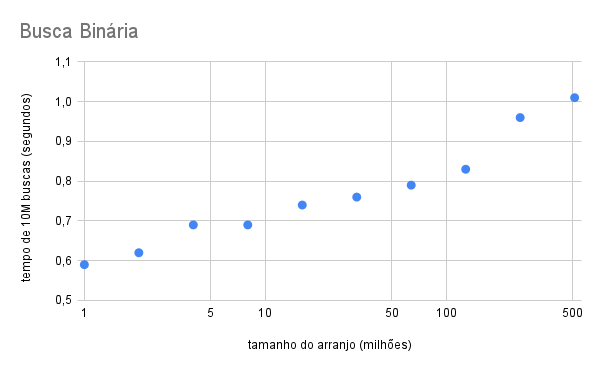
\includegraphics[width=0.9\textwidth]{imagens/grafico4.png}
  \caption{Gráfico ilustrando a hipótese de que o tempo de processamento da busca binária segue a função constante $t(2^y) = a.y + b$.}
\end{figure}

Como fizemos no exemplo anterior, podemos computar os valores de $a$ e $b$ utilizando uma técnica de regressão linear.
Ficamos assim com $a = 0,043$ e $b = 0,529$.

Por fim, mudamos a variável $2^y = x$ e obtemos a seguinte equação:

\begin{displaymath}
  t(x) = a.log_2(x) + b = 0,043.log_2(x) + 0,529
\end{displaymath}

